% !TEX root=../../deissue.tex 


% 1 Introduction:

% 1.1 Describe challenges of COVID-19.

% 1.2 How to address these challenges. 

% 1.3 A data-science pipeline. Data discovery, data integration and cleaning, automatic visualization, efficient tracking and searching (china mobile), trend prediction/search

% 1.4 Contributions:

% 2 System architecture

% 3 Data preparation 

% 4 Automatic Visualization.

% 5 Efficient tracking and searching å

% 6 Trend prediction

% \documentclass[11pt]{article}
% \usepackage{deauthor,times,graphicx}

% \newcommand{\G}{\mathcal{G}}
% \newcommand{\C}{\mathcal{C}}
\newcommand{\Q}{\mathcal{Q}}
\newcommand{\V}{\mathcal{V}}
\newcommand{\E}{\mathcal{E}}
\newcommand{\A}{\mathcal{A}}
\newcommand{\I}{\mathcal{I}}
\newcommand{\Rels}{\mathcal{R}}
\newcommand{\score}{\texttt{score}}
\newcommand{\rank}[1]{\texttt{Rank}(#1)}
\newcommand{\den}[1]{\llbracket #1 \rrbracket}
\newcommand{\oden}[1]{\llbracket #1 \rrbracket_{\textrm{train}}}


\newcommand{\Em}[1]{f_\theta({#1})}

\newcommand{\ea}{\emph{et al.}}
\newcommand{\eg}{\emph{e.g.}}
\newcommand{\ie}{\emph{i.e.}}
\newcommand{\iid}{\emph{i.i.d.}}
\newcommand{\etc}{\emph{etc.}}

\newcommand{\R}{\mathbb{R}}
\newcommand{\RR}{\mathbb{R}}
\newcommand{\CC}{\mathbb{C}}
% \newcommand{\mb}{\mathbf}
\newcommand{\Proj}{\mathcal{P}}
\newcommand{\Inter}{\mathcal{I}}

\newcommand{\xhdr}[1]{{\noindent\bfseries #1}.}
\newcommand{\CITE}{{\textcolor{red}{CITE}}}
\newcommand{\cut}[1]{}
\newcommand{\name}{GQE}
\newcommand{\newparagraph}[1]{\vspace{2pt}\noindent\textbf{#1}}

\newcommand{\distt}[3]{{{\texttt{Dist}(#1, #2, #3)}}}
\newcommand{\distr}[3]{{{\texttt{Residue}(#1, #2, #3)}}}


\newcommand{\dq}{\llbracket q\rrbracket}
\newcommand{\dqp}{\llbracket q'\rrbracket}
\newcommand{\dqone}{\llbracket q_1\rrbracket}
\newcommand{\dqtwo}{\llbracket q_2\rrbracket}
\newcommand{\dqtr}{\llbracket q\rrbracket_\texttt{train}}
\newcommand{\dqv}{\llbracket q\rrbracket_\texttt{val}}
\newcommand{\dqte}{\llbracket q\rrbracket_\texttt{test}}
\newcommand{\dqx}{\llbracket q\rrbracket_\text{extra}}
\newcommand{\dqitr}{\llbracket q_i\rrbracket_\text{train}}
\newcommand{\dqiv}{\llbracket q_i\rrbracket_\text{val}}
\newcommand{\dqite}{\llbracket q_i\rrbracket_\text{test}}
\newcommand{\dqix}{\llbracket q_i\rrbracket_\text{extra}}
\newcommand{\qp}{q_\text{path}}
\newcommand{\Qp}{Q_\text{path}}
\newcommand{\qc}{q_\text{conj}}
\newcommand{\Qc}{Q_\text{conj}}
\newcommand{\Gtr}{\G_\text{train}}
\newcommand{\Gte}{\G_\text{test}}
\newcommand{\Gv}{\G_\text{valid}}
\newcommand{\Etr}{\E_\text{train}}
\newcommand{\Ete}{\E_\text{test}}
\newcommand{\Ev}{\E_\text{valid}}

\newcommand{\Emb}[1]{\text{Em}(#1)}
% \newcommand{\Ce}{\text{Cen}}
% \newcommand{\Of}{\text{Off}}

% \newcommand{\Em}[1]{\mathbf{#1}}
% \newcommand{\Em}[1]{\mathbf{#1}}
\newcommand{\Emint}[1]{\mathbf{#1_\texttt{Inter}}}
\newcommand{\pEm}[1]{p_\mathbf{#1}}
\newcommand{\pEmint}[1]{p_\mathbf{#1_\texttt{Inter}}}
\newcommand{\Ce}[1]{\text{Cen}(#1)}
\newcommand{\Of}[1]{\text{Off}(#1)}
\newcommand{\exec}[1]{\textsc{LSE}(#1)}

\newcommand{\q}[1]{\textsc{#1}}

\newcommand\qu[1]{``\emph{#1}''}

% \newtheorem{theorem}{Theorem}
% \newtheorem{definition}{Definition}
% \newtheorem{corollary}{Corollary}
% \newtheorem{proposition}{Proposition}
\newtheorem{observation}{Observation}
% \newtheorem{lemma}{Lemma}
\newtheorem{rem}{Remark}

% \makeatletter           

\begin{document}

\title{\textsc{DeepEye}: A Data Science System for Monitoring and Exploring COVID-19 Data}

\author[${\dag}$]{Yuyu Luo}
\author[${\ddag}$]{Nan Tang}
\author[${\dag}$]{Guoliang Li}
\author[${\dag}$]{Wenbo Li}
\author[${\dag}$]{Tianyu Zhao}
\author[${\dag}$]{Xiang Yu}
\affil[${\dag}$]{Department of Computer Science, Tsinghua University}
\affil[${\ddag}$]{Qatar Computing Research Institute, HBKU}
\affil[ ]{\small \{luoyy18@mails., liguoliang@, li-wb17@mails., zhaoty17@mails., x-yu17@mails.\}tsinghua.edu.cn, ntang@hbku.edu.qa}

% \author{ \hspace{-1em} %\alignauthor 
% 	Yuyu Luo$^{\dag}$\hspace{1em}
% 	Nan Tang$^{\ddag}$\hspace{1em} 
% 	Guoliang Li$^{\dag}$\hspace{1em}
% 	Wenbo Li$^{\dag}$\hspace{1em}
% 	Tianyu Zhao$^{\dag}$\hspace{1em}
% 	Xiang Yu$^{\dag}$
% 	\\
% \affaddr{\small$^{\dag}$Department of Computer Science, Tsinghua University \hspace{2ex} $^{\ddag}$Qatar Computing Research Institute, HBKU} \\
% \hspace{-1em}
% 	{\small \{luoyy18@mails., liguoliang@, li-wb17@mails., zhaoty17@mails., x-yu17@mails.\}tsinghua.edu.cn, ntang@hbku.edu.qa}
% }


\maketitle

The recent surge in blockchain applications has accelerated the research in 
designing efficient decentralized currencies. Building a decentralized economy 
on the traditional byzantine fault-tolerant (\BFT{}) protocols or the Proof-of-Work 
(\PoW{}) consensus protocol is inadequate as the immutability of the ledger created 
by the former is at the mercy of the long-term safe-keeping of private keys of 
participants, while the latter yields an extremely inefficient and environmentally 
unsustainable consensus. To ameliorate this situation, we envision the design of 
our \DualChain{} architecture, which offers the best of both worlds. Our \DualChain{} 
design runs a traditional \BFT{} protocol to commit client transactions and employs 
our novel Power-of-Collaboration (\PoC{}) protocol to notarize the \BFT{} chain. 
Unlike \PoW{}, our \PoC{} protocol advocates for participants to work together 
collaboratively instead of competing (often selfishly), which results in a 
safe, high-throughput, and resource-efficient consensus design.


\section{Introduction}

Information Retrieval (IR) involves retrieving a set of candidates from a large document collection
given a user query. The retrieved candidates may be further reranked to bring the most relevant ones to the top, constituting a typical retrieve-and-rerank (R\&R) framework \cite{wang2018evidence, hu2019retrieve}.
Reranking generally improves the ranks of relevant candidates among those retrieved, thus improving on metrics such as Mean Reciprocal Rank (MRR) \cite{Craswell2009} and Normalized Discounted Cumulative Gain (nDCG) \cite{jarvelin2002cumulated}, which assign better scores when relevant results are ranked higher. 
However, retrieval metrics like Recall@K, which mainly evaluate the presence of relevant candidates in the top $K$ retrieved results, remain unaffected.
Increasing Recall@K can be key, especially when the retrieved results are used in downstream knowledge-intensive tasks \cite{petroni2021kilt} such as open-domain question answering \cite{chen2017reading, chen2020open, gangi2021synthetic}, fact-checking \cite{thorne2018fever}, entity linking \cite{hoffart2011robust,sil2013re,sil2018neural} and dialog generation \cite{dinan2018wizard, komeili2022internet}.

Most existing neural IR methods use a dual-encoder retriever \cite{karpukhin2020dense, khattab2020colbert} and a subsequent cross-encoder reranker \cite{nogueira2019passage}. 
Dual-encoder\footnote{We use the terms bi-encoder and dual-encoder interchangeably in this paper.} models leverage separate query and passage encoders and perform a late interaction between the query and passage output representations. This enables them to perform inference at scale as passage representations can be pre-computed. Cross-encoder models, on the other hand, accept the query and the passage together as input, leaving out scope for pre-computation. The cross-encoder typically provides better ranking than the dual-encoder---thanks to its more elaborate computation of query-passage similarity informed by cross-attention---but is limited to seeing only the retrieved candidates in an R\&R
framework.


\begin{wrapfigure}{r}{0.42\linewidth}
    \centering
    \includegraphics[width=1.0\linewidth]{submissions/Revanth2024/figures/cross_encoder_feedback_2.png}
    \caption{\textsc{ReFIT}: The proposed method for reranker relevance feedback. We introduce an inference-time distillation process (step 3) into the traditional retrieve-and-rerank framework (steps 1 and 2) to compute a new query vector, which improves recall when used for a second retrieval step (step 4).}
    \label{fig:overall_framework}
    \vspace{-1em}
\end{wrapfigure}

Since the more sophisticated reranker often generalizes better at passage scoring than the simpler, but more efficient retriever, here we propose to use relevance feedback from the former to improve the quality of query representations for the latter directly \textit{at inference}.
Concretely, after the R\&R pipeline is invoked for a test instance, we update the retriever's corresponding query vector by minimizing a distillation loss that brings its score distribution over the retrieved passages closer to that of the reranker.
The new query vector is then used to retrieve documents for the second time. 
This process effectively teaches the retriever how to rank passages like the reranker---a stronger model---for the given test instance.
Our approach, \textsc{ReFIT}\footnote{\textsc{ReFIT} stands for \textbf{Re}ranker \textbf{F}eedback at \textbf{I}nference \textbf{T}ime}, is lightweight as only the output query vectors (and no model parameters) are updated, ensuring comparable inference-time latency when incorporated into the R\&R framework. 
Figure \ref{fig:overall_framework} shows a schematic diagram of our approach, which introduces a distillation and a second retrieval step into the R\&R framework.
By operating exclusively in the representation space---as we only update the query vectors---our framework yields a parameter-free and architecture-agnostic solution, thereby providing flexibility along important application dimensions, e.g., the language, domain, and modality of retrieval. 
We empirically demonstrate this effect by showing improvements in retrieval on multiple English domains, across 26 languages in multilingual and cross-lingual settings, and in different modalities such as text and video retrieval.
 

Our main contributions are as follows:
\begin{itemize}
    \item We propose \textsc{ReFIT}, an inference-time mechanism to improve the recall of retrieval in IR using relevance feedback from a reranker.
    \item Empirically, \textsc{ReFIT} improves retrieval performance in multi-domain, multilingual, cross-lingual and multi-modal evaluation.
    \item The proposed distillation step is fast, considerably increasing recall without any loss in ranking performance over a standard R\&R pipeline with comparable latency.
\end{itemize}



%!TEX root = ../main.tex
\section{An Overview of DeepEye}
\label{sec:system}

\subsection{System Architecture}

%\add{Rename the layers to be consistent with Introduction.}
We present \sys, an end-to-end framework to prepare data, select visualizations and allow easy-to-use interactions. An overview of \sys is given in Figure~\ref{fig:framwork}, which consists of three layers: {\em (task-driven) data preparation layer}, {\em (smart) data analytics layer}, and {\em user interaction layer}.
%
%\add{!!!!}
%
Data preparation is responsible for crawling daily updated data from different sources, and cleaning them when needed (Section~\ref{subsec:dp}).
%
Data analytics describes the process of both which charts will always be shown (\eg a heat map on a world map showing new cases of every country), and how to automatically recommend visualizations that are ``interesting'' \wrt new incoming data, for visual analytics (Section~\ref{subsec:vs}).
%
Interaction allows a user to explore various and (maybe) new COVID-19 stories in an interactive fashion (Section~\ref{subsec:ie}).


\subsection{Task-driven Data Preparation Layer}
\label{subsec:dp}

%%%%%%%%%%%%%%%%%%%%%%%%%%%%%%%%%%%%
\begin{figure}[t!]
	\centering
	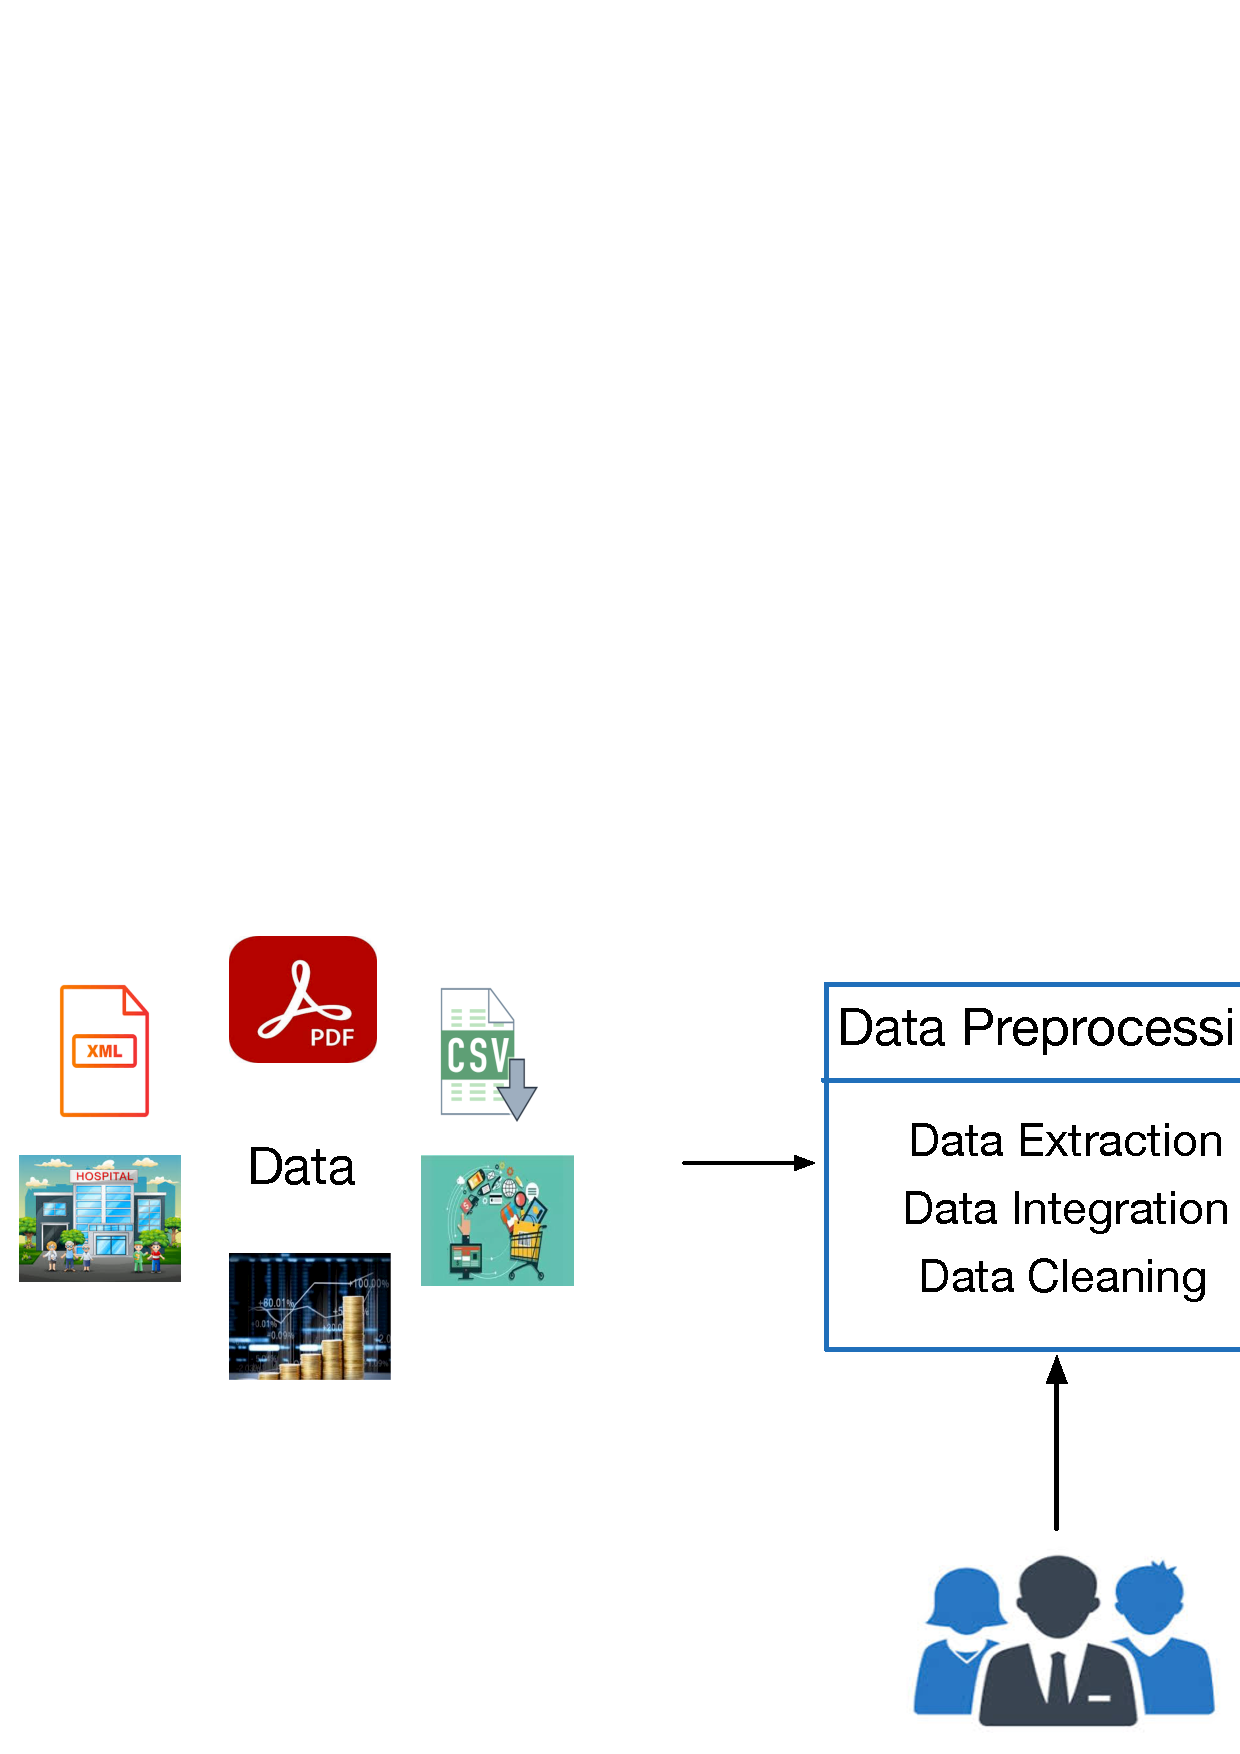
\includegraphics[width=.6\columnwidth]{figs/framework.pdf}
	\caption{System Overview}
	\label{fig:framwork}
\end{figure}
%%%%%%%%%%%%%%%%%%%%%%%%%%%%%%%%%%%%


This layer has a predefined pipeline to prepare data, which will run periodically, with the following three steps.

\stitle{Data Collection.}
We collect data from the following data sources.
(1) We download hourly the official data from the Chinese Center for Disease Control and Prevention (CDC) and other countries' CDCs.
(2) We crawl infected cases' age and gender from authoritative news websites.
(3) We also connect to other data sources like population statistics, temperature data, and so on. 
(4) We are also provided with trajectory data of (potentially) infected persons from China Mobile Limited\footnote{We are collaborating with the company and got mobile phone location data under privacy protection.}. 
%The schema is {\sf S1:}({\sf PhoneID}, {\sf Tag}, {\sf Province}, {\sf City}, {\sf District}, {\sf Address}, { \sf Longitude}, {\sf Latitude}, {\sf Time}).

\stitle{Data Integration.} Next, we need to integrate different types of data into predefined relational tables (\ie global views).
For example, we need to extract report date, location, patients' type, \#-cases from each country's CDC's reports, and  perform schema alignment into  $S1$: ({\em Date, Country, State/Province, City, Total Confirmed, Active Confirmed, Total Deaths, Total Recovered, Death Rate, Recovered Rate, Gender)}, a typical ETL-based data integration process. 


\stitle{Data Cleaning.} After integrating data from multiple sources, there have typical data errors such as duplicates, missing values, synonyms, and so on. 
%\add{Add a sentence to say that we will discuss task-driven data cleaning in Section 3.}
Because data cleaning is known to be tedious and error-prone, we employ our recently proposed technique {\sc VisClean}~\cite{visclean-icde} for visualization-aware data cleaning, which is way cheaper than cleaning the entire dataset. This is doable only after the charts to display have been selected, as discussed below. 
We will depict more details about visualization-aware data cleaning in Section~\ref{sec:dataprep}.

\subsection{Smart Data Analytics Layer}
\label{subsec:vs}
Based on the availability and reliability of data and meta-data, we have successfully conducted the following types of data analytics.

\stitle{Descriptive analytics.} 
We use linked data visualization and visualization recommendation algorithms to effectively show what happened in the past.


\stitle{Diagnostic analytics.} 
We use maps with different layers to test the spatio-temporal properties of COVID-19 data, especially to show the effect of urban (population) density and temperature to the outbreak of COVID-19.


\stitle{Prescriptive analytics.}
Based on the collaboration with companies to get private data, we were able to do some meaningful prescriptive analytics that can recommend actions to decision makers.

%%%%%%%%%%%%%%%%%%%%%%%%%%%%%%%%%%%%
%\begin{figure}[t!]
%	\centering
%	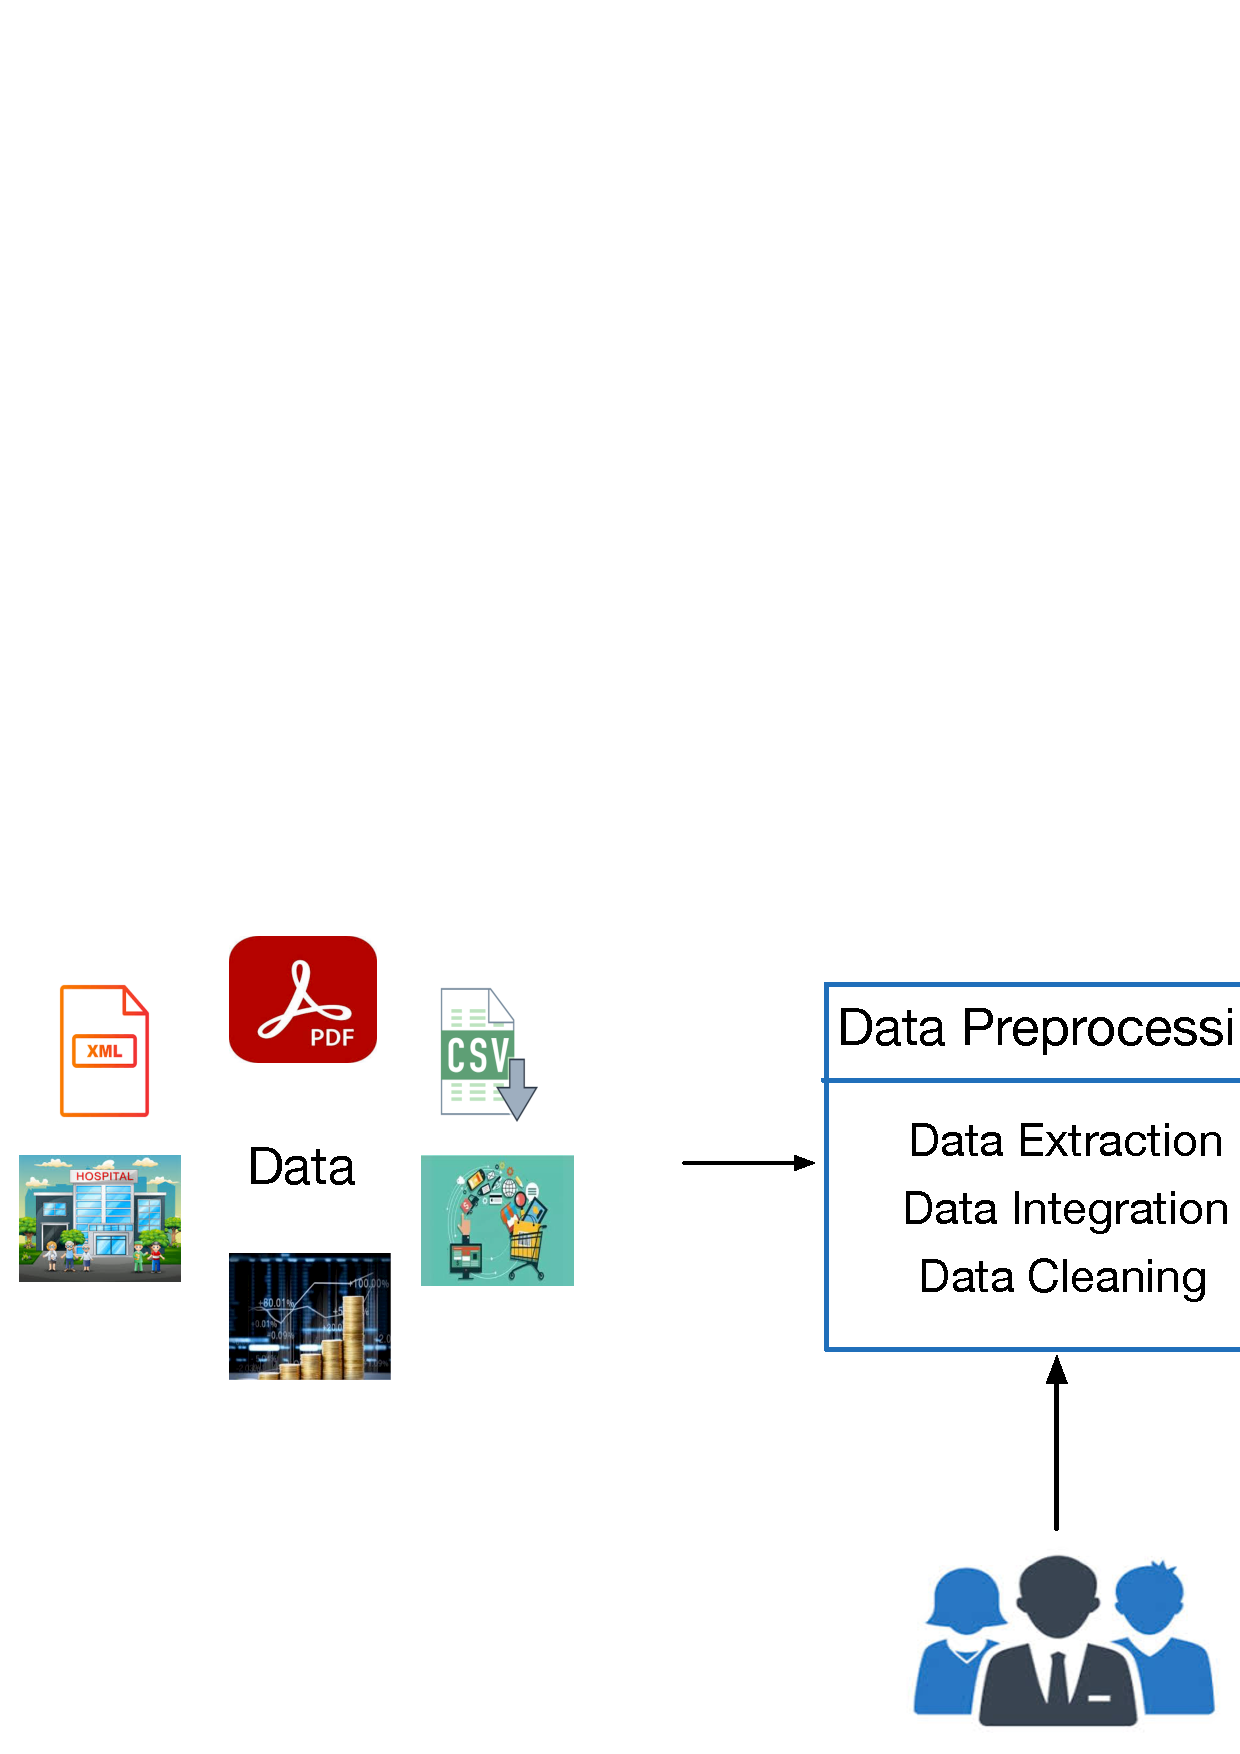
\includegraphics[width=.6\columnwidth]{figs/framework.pdf}
%	%	\vspace{-1.5em}
%	\caption{System Overview}
%	\label{fig:framwork}
%	%	\vspace{-2.5em}
%\end{figure}
%%%%%%%%%%%%%%%%%%%%%%%%%%%%%%%%%%%%





%%%%%%%%%%%%%%%%%%%%%%%%%%%%%%%%%%%%
%\begin{figure*}[t!]
%	\vspace{-1.5em}
%	\centering
%	\includegraphics[width=0.9\textwidth]{figs/frontend.pdf}
%	%	\vspace{-1.5em}
%	\caption{Demonstration of \sys-COVID-19 (https://ncov.deepeye.tech/en)}
%	\label{fig:frontend}
%	%	\vspace{-1.5em}
%\end{figure*}
%%%%%%%%%%%%%%%%%%%%%%%%%%%%%%%%%%%%


% \stitle{\sys-COVID-19:}
% We have implemented a \sys instance for COVID-19, which has attracted a broad range of interest from general users, public health authorities, and researchers who want to explore the COVID-19 data and track the outbreak. 
% %


% The base view of \sys-COVID-19 is shown in Figure~\ref{fig:frontend}, which consists of a choropleth map for the total confirmed/recovered/died cases for all countries, line charts for the trend of daily increased cases, calendar charts for visualizing the types of patients, bar charts for distributions of patients' ages, bubble charts for cure rate - death rate, and so on. 
% %
% Besides the basic view page, it also has ad-hoc features, such as tracking infection path and high-risk areas discovery using the trajectory data of infected persons, which will be discussed in Section~\ref{sec:demo}.


% \sys has three layers (see Figure~\ref{fig:framwork}): (1) data preparation, (2) visualization selection, and (3) interaction.
% Next, we will explain each step using the COVID-19 case.


% %%%%%%%%%%%%%%%%%%%%%%%%%%%%%%%%%%%%
% \begin{figure*}[t!]
% 	\centering
% 	\includegraphics[width=0.9\textwidth]{figs/frontend.pdf}
% 	\caption{Demonstration of \sys-COVID-19 (\lgl{https://ncov.deepeye.tech/en})}
% 	\label{fig:frontend}
% 	\vspace{-.5em}
% \end{figure*}
% %%%%%%%%%%%%%%%%%%%%%%%%%%%%%%%%%%%%






%The data preparation layer, an end-to-end data preparation pipeline, is responsible for collecting, integrating, and cleaning data from multiple data sources. 
%There are some common obstacles in the implementation of this layer. 
%First, we needs to 
%In our application, we collect the reported infected cases from the Chinese Center for Disease Control and Prevention (CDC) and other countries' CDC, and crawler infected cases' age and gender from authoritative news websites, and other data sources like Chinese population statistics.  Moreover, we also gather trajectory data of (potentially) infected persons from China Mobile Limited\footnote{We have collaborated with the company and got mobile phone location data with privacy protection.}. The schema is {\sf S1:}({\sf PhoneID}, {\sf Tag}, {\sf Province}, {\sf City}, {\sf District}, {\sf Address}, { \sf Longitude}, {\sf Latitude}, {\sf Time}).

%Next, we need to integrate different types of data into the relational table.
%For example, we need to extract report date, location, patients' type, \#-cases from each country's CDC's reports, and  perform schema alignment into {\sf S2:}({\sf Date}, {\sf Country}, {\sf State/Province}, {\sf City}, {\sf Total Confirmed}, {\sf Current Confirmed}, {\sf Total Deaths}, {\sf Total Recovered}, {\sf Death Rate}, {\sf Recovered Rate}, {\sf Gender}).

% \stitle{Data Cleaning.} After integrating data from multiple sources, there have typical data errors such as duplicates, missing values, synonyms, and so on. Because data cleaning is known to be tedious and error-prone, we employ our recently proposed technique {\sc VisClean}~\cite{visclean-icde} for visualization-driven data cleaning, which is way cheaper than cleaning the entire dataset. This is doable only after the charts to display have been selected, as discussed below.

%In the above steps, it may introduce some data errors such as duplicates, missing values, and synonyms. 
%Such errors may derive bad visualizations and may misguide users by showing false discoveries. 
%It's necessary to clean the data errors before conduct analysis. However, it is impossible to completely clean a dataset for visualizations (or any other analytical task), simply because data cleaning is prohibitively expensive in terms of the human cost.
%Therefore, we propose to clean those data errors that are relevant to the analysis~\cite{visclean-icde}.

%The system can automatically rerun the pipeline to update data to guarantee its timeliness. 
%Once the pipeline is built, and the data is ready, the next step is to analyze and visualize the data.

% \subsection{Visualization Selection Layer}
% \label{subsec:vs}

% % \add{Paragraph 1: Two types of visualizations are needed. General statistics/trends that can be fixes, and data-driven interesting charts that may be different everyday. So you have Sections 2.2.1 and 2.2.2.}

% Visualization selection generates three categories of charts: {\em linked} common visualizations, {\em ad-hoc} visualizations, and {\em recommended} visualizations.

% \stitle{Linked Common Visualizations.} There are common visualizations for spatial-temporal data exploration, such as a choropleth map (a heat map on a map), line charts to show various trends, bar charts to show the comparison between various groups, scatter charts (or bubble charts) to quantify the relationship between two quantitative variables (\eg death rate vs. cure rate).
% We carefully selected charts (see Figure~\ref{fig:frontend}) that can attract a wide range of interest, and make them ``linked'', \eg when one zoom in from a world level to a country level, all the other charts will be zoomed in, so as to provide a synchronized view from multiple charts.

%%%%%%%%%%%%%%%%%%%%%%%%%%%%%%%%%%%%
\begin{figure}[t!]
	\centering
	\includegraphics[width=.9\columnwidth]{figs/drill_down_new.pdf}
	\vspace{-1.5em}
	\caption{Drill Down Operation}
	\label{fig:drill_down}
	%	\vspace{-1.5em}
\end{figure}
%%%%%%%%%%%%%%%%%%%%%%%%%%%%%%%%%%%%



\subsection{User Interaction Layer}
\label{subsec:ie}
This is the interface we present to the public.
When a user visits \sys, he/she can further explore visualizations by interactive module for finding more interesting insights. \sys supports popular interactions such as drilling down/up, zooming in/out and linked visualizations, powered by the visualization library ECharts~\cite{DBLP:journals/vi/LiMSSZWZC18}.

Take drill down as an example (see Figure~\ref{fig:drill_down}), when a user clicks a country (\eg China) on the world-level map, the map will drill down into the country-level map for more details.
Note that, \sys provides linked visualizations of the analytical results. That is, when a user performs a drill down operation, other visualizations will also drill down into certain level automatically. In addition, the user can zoom in/out the map by rolling up/down the mouse. 



%It consists of two components, \ie data-dependent visualization design and visualization recommendation. The key points in this layer are (1) what types of visualizations should be designed to interpret the underlying data best; and (2) how to generate such visualizations effectively because there 

% \subsubsection{Data-dependent  Visualization Design}
% For temporal data, there are several common types of visualizations are needed.
% The first type of visualization is line chart, it shows the trend of the temporal data. The second one is bar chart, it shows the distribution or compared information of variables of temporal data, \eg the distribution of the patients' ages.
% Scatter chart (or bubble chart) discovers and quantifies the relationships between two quantitative variables, \eg the death rate v.s. cure rate. 


% \add{Paragraph 1: Maybe you should not call it analysis models, which is not very informative. It should be something like data-dependant chart design or selection, from common ones to special ones, such as infection path or location-based search.}

% It includes a set of data analytical models to process the data for visualization. The analytical models take data as input and output analytical for visualization.
% We implement four types of analysis models in the system. 
% Note that data analysts can plug their analytical model with their domain knowledge into the system, \eg mining the relationships between death rate and medical resources.

% \stitle{Aggregation Analysis.}
% We apply the aggregation analysis to aggregate relational data for visualization. For example, we can use compute the total confirmed cases for each country.

% \stitle{Correlation Analysis.}
% It discovers and quantifies the relationships between two quantitative variables. For example, we can analyze the relationships between \#-cases and recovery (death) rate.

% \stitle{Trend Analysis.}
% For one thing, it records the trend of variables. For another, it can try to predict what will happen in the future.
% In our scenario, we can show the trend of daily increased cases for each country and predict the trend for the coming days. In our system, we use a two-layer neural network $f$ to predict the number of daily confirmed cases in China. The incubation period of the corona virus is 14 days, so we choose the data from the previous 14 days $x=\{c_{-1},c_{-2},...,c_{-14}\}$ as the first input feature and the date of the next day $d$ as the second input feature. We predict the total number of confirmed cases $c = f (x, d)$ the next day. Inspired by the traditional infectious disease model SIR~\cite{kermackcontribution}, we use sigmoid as the activation function in our model $f$.  Gradient descent is used to update the parameters of $f$. By continuously taking the predicted value of the next day as an input, we can continuously predict the confirmed cases in the following days.

% \stitle{Ad-hoc Visualizations}. We also design ad-hoc visualizations to answer specific questions. In terms of COVID-19, besides publicly available datasets, we also have private trajectory data of potentially infected persons. Based on which we have designed two map-based visualizations, one to show infection paths of these patients (see Figure~\ref{fig:infection}), and the other to show the level of risk for each area (see Figure~\ref{fig:heatmap}) and thus suggest the authorities to take different anti-epidemic policies for different areas.

%Besides the above four types of common visualizations, we also need to design some visualizations relevant to analysis scenario.
%Since we also collect the trajectory data of (potential) infected persons.
%Therefore, we use the map to visualize the trajectories. It can benefit us to find such potential infected persons visually, and perform a trajectory similarity search to find a set of similar trajectories to the trajectories of (potential) infected persons. Therefore, we can find a set of high-risk groups. Based on the above analysis, we can further compute the level of risk for each area and thus suggest the authorities take different anti-epidemic policies for different areas.


%\subsubsection{Visualization Recommendation}

% \add{Paragraph 1: Emphasize the requirement of daily news, instead of only daily updates. Why it is hard to have daily news -- a large search space. Naturally, we need some recommendation systems to guide us for doing the job, and we use DeepEye.}

% \stitle{Recommended Visualizations}.
% The above common visualizations are fixed, with data being periodically updated. However, because the data keeps changing, and some interesting stories cannot be captured by predefined common visualizations. Hence, it requires some mechanism to discover these new interesting visualizations, either manually or automatically.
% We leverage our previous work, a visualization recommendation system called {\sc DeepEye}~\cite{deepeyeicde}, to recommend interesting visualizations, such as finding cities in China that share similar trends as Wuhan in terms of death rate. 
% The basic idea of {\sc DeepEye} is to take a table as input, enumerates all possible visualizations of the dataset, select those good visualizations by a supervised classification model, and ranks top-$k$ good visualizations by a learning-to-rank model.

%After we know use what types of visualizations to interpret the data, the next problem is how to process the data for visualization. Not surprisingly, creating good visualizations is not easy in practice, even for the expert. The reason is that it requests the analyst to understand the data both from statistic and semantic perspectives, the right combination of attributes and the right selection of subset. Moreover, the temporal data is usually updated in a certain time interval, and the data feature may also be changed. Thus, the goodness of data-driven visualizations are highly dependent on underlying data.  Therefore, how to select a set of good visualizations after data updating is also a challenge.

%To alleviate the above problem, we propose to use a hybrid method to generate and select good visualizations for the data.  First, we select a set of good visualizations leveraging our previous work, a visualizations recommendation system~\cite{deepeyeicde}. The basic idea of the system is that it takes a relational dataset as input, enumerates all possible visualizations the dataset, select those good visualizations by a classification model, and ranks top-$k$ good visualizations by a learning-to-rank model. Second, we also can manually design good visualizations by incorporating domain knowledge and analysis targets for the dataset. For example, we design a Spatio-temporal choropleth map (\ie choropleth map in Figure~\ref{fig:frontend}) to track the outbreak of COVID-19 around the world visually.  Thus, we select a group of novel visualizations based on the above method and organize those visualizations as a dashboard (See Figure~\ref{fig:frontend}).

% \subsection{Interaction Layer}
% \label{subsec:ie}

% \add{Paragraph 1: You can give some details about the tools you use to implement such a system.}

%Second, what kinds of interactions should we support to enable the visual exploration process more user-friendly.

%\subsection{Interactive Visualization}
%The users also can interact with visualizations to explore the data. 
%
%zoom in, zoom out
%
%drill down, drill up
%
%time line tracking
%
%linking across multiple visualizations

% \stitle{Interaction Types.}

% %%%%%%%%%%%%%%%%%%%%%%%%%%%%%%%%%%%%
% \begin{figure}[t!]
% 	\centering
% 	\includegraphics[width=.75\columnwidth]{figs/drill_down.pdf}
% 	\vspace{-1.5em}
% 	\caption{Drill Down Operation}
% 	\label{fig:drill_down}
% %	\vspace{-1.5em}
% \end{figure}
% %%%%%%%%%%%%%%%%%%%%%%%%%%%%%%%%%%%%
% %%%%%%%%%%%%%%%%%%%%%%%%%%%%%%%%%%%%%
% \begin{figure}[t!]
% 	\centering
% 	\includegraphics[width=.75\columnwidth]{figs/similarity_trend1.pdf}
% 	\caption{Similar Trend of Confirmed Cases}
% 	\label{fig:similar_trend}
% \end{figure}
% %%%%%%%%%%%%%%%%%%%%%%%%%%%%%%%%%%%%

% \subsection{Interactive Visualization}

% This is the interface we present to the public. 
% When a user visits \sys, he/she can further explore visualizations by interactive module for finding more interesting insights. \sys supports popular interactions such as drilling down/up, zooming in/out and linked visualizations.

% Take drill down as an example (see Figure~\ref{fig:drill_down}), when a user clicks a country (\eg China) on the world-level map, the map will drill down into the country-level map for more details.
% Note that, \sys provides linked visualizations of the analytical results. That is, when a user performs a drill down operations, other visualizations will also drill down into certain level automatically. In addition, the user can zoom in/out the map by rolling up/down the mouse.



% \subsection{How to support reuse and plugin.}
% \label{subsec:disscussion}


%!TEX root = ../main.tex
\section{Human-in-the-loop Machine Learning Pipeline}
\label{sec:pipeline}

As shown in Figure~\ref{fig:framwork}, humans play significant roles in machine learning pipeline. First, given some unstructured data, we have to transform it structured data, in order to construct features for ML. Then for structured data from multiple sources, we should integrate them for enriching data and features to achieve  well-performed ML model. What's more, data is always dirty in the real world. To further improve the performance, we should clean the data, such as repairing records that violate integrity constraint  and  removing outliers and duplicates. Finally, we should annotate the data for building the model. For all above steps in the pipeline, humans can contribute their intelligence to provide high quality training data and improve the ML model. Next, we will introduce what humans can contribute in these steps.



\subsection{Data Extraction}

Extracting structured data from unstructured data is an important problem both in industry and academia, which has been studied broadly from rule-based~\cite{DBLP:conf/acl/LiRC11} systems to ML-based  approaches~\cite{DBLP:conf/wsdm/NakasholeTW11, DBLP:conf/aaai/MitchellCHTBCMG15}. However, these methods either need domain experts to design rules or humans to provide large quantities of labels. Recently, DeepDive~\cite{DBLP:conf/sigmod/Zhang0RCN16} is a representative system in this area, which provides  declarative language  for  non-expert users to extract data.  The execution of DeepDive can be divided into three parts: candidate generation, supervision, statistical inference and learning. Humans mainly contribute in the first part, i.e., candidate generation. In this part, humans write some extraction rules described by declarative languages to retrieve data with attributes or relations, such as  entity B is the wife of A if there exists mention ``and his wife" between A and B in a corpus. The goal of this part is to generate candidates with high recall and low precision. Secondly, the supervision part applies distant supervision rules from knowledge bases or incomplete databases  to provide labels for some of the candidates. The rules do not need to label all candidates from the first part, which are intended to be a low recall and high precision. For the last part, DeepDive constructs a graphical model that represents all of the labeled candidate extractions, trains the model, and then infers a correct probability for each candidate. At the end of this stage, DeepDive applies a threshold to each inferred probability and then derives the extractions to  the output database. In conclusion, Deepdive leverages humans to provide extraction candidates with high recall, uses weak supervision(distance supervision) to label them and finally trains a statistical ML model to fine-tune the labels.
 
 

\subsection{Data Integration}
Given relational tables from multiple sources, in many cases we want to integrate them for extending existing datasets, including features and records. To this end, schema matching~\cite{DBLP:journals/pvldb/ZhangCJC13,DBLP:conf/icde/FanLOTZ14} and entity resolution~\cite{DBLP:crowder, DBLP:transitivity} have to be applied, where the first part is going to align the columns and the second will match records from different tables. Recently, many existing works focused on leveraging human intelligence to achieve these. 

For schema matching, existing works~\cite{DBLP:journals/pvldb/ZhangCJC13} utilize human-machine hybrid approaches to improve the performance. They utilize machine-based  schema matching tools to generate a set of possible matchings, each of which has a probability to be matched. 
They define a correspondence correctness question (CCQ) for humans to answer, which denotes a pair of attributes from two columns, so each matching consists of a set of correspondences. Then the problem is to wisely choose  the correspondences to ask the human to obtain the highest certainty of correct schema matching at the lowest cost. The uncertainty is measured by entropy on top of the probabilities that the tools generate. 
In the correspondence selection, they consider the column correlations, selection efficiency and human quality to match schemes effectively and efficiently. 
Fan et.al~\cite{DBLP:conf/icde/FanLOTZ14} introduce knowledge base together with humans to do schema matching. First, they propose a concept-based approach that maps each column of a  table to the best concept in knowledge bases. This approach overcomes the problem that sometimes values of two columns may be disjoint, even though the columns are related, due to incompleteness in the column values. Second, they develop a hybrid machine-crowdsourcing framework that leverages human intelligence to discern the concepts for ``difficult'' columns. The overall framework assigns the most ``beneficial'' column-to-concept matching tasks to the human under a given budget and utilizes the answers to  infer the best matching. 

After the schemes are aligned, we can integrate different relational tables by the join operation. Traditionally, join is always executed by exact matching between values of attributes from two tables. However, in the real world,  data is  always dirty. For example, ``Apple iPhone 8" and "iPhone 8th" refer to the same entities and should be joined, which cannot be done by a traditional database. Therefore, the human-based join is proposed to address this problem. Wang et.al.~\cite{DBLP:crowder} propose  crowd-based join framework, which generates many candidate pairs, uses similarity based pruning techniques to eliminate dissimilar pairs and ask the crowd to answer the rest  pairs. To further reduce the cost, Wang et.al.~\cite{DBLP:transitivity} leverage the transitivity technique to deduce unknown answers based on current answers from humans. Chai et.al.~\cite{DBLP:journals/vldb/ChaiLLDF18, DBLP:conf/sigmod/ChaiLLDF16} build a partial-order graph based on value similarities of different attributes and utilize the graph to prune pairs that are not necessary to ask. To improve the quality,  Wang et.al.~\cite{DBLP:conf/sigmod/WangXL15} first cluster the entities to be joined  and then leverage humans to refine the clusters. Yalavarthi et.al.~\cite{DBLP:conf/cikm/YalavarthiKK17} select questions judiciously considering the crowd errors.





\subsection{Data Cleaning}

Data is dirty in the real world, which is likely to hurt the ML performance. For example, some values may be out of range (e.g., age is beyond 120 or below 0) or utilize wrong units (e.g., some distances are in meters while other are in kilometers); Some records  refer to the same entity; Integrity constraints (e.d. functional dependencies) are violated among records. Recently, many researchers focused on leveraging human to clean the data. For instance, crowd-based entity resolution~\cite{DBLP:crowder, DBLP:journals/vldb/ChaiLLDF18, DBLP:conf/sigmod/ChaiLLDF16} is applied  to remove duplicates. Chai et.al. ~\cite{DBLP:conf/sigmod/ChaiC00LM20} use human expertises to identify outliers among the data. Specifically, they first utilize machine-based outlier detection algorithms to detect some outlier candidates as well as inlier candidates, and then human is asked to verify these candidates by comparing outlier candidates with inliers.  Chu et.al.~\cite{DBLP:journals/pvldb/ChuOMIP0Y15} clean the  data that violates integrity constraints with the help of knowledge base and humans. They first identify the relationships between columns using knowledge base and then use humans to verify them. Then the discovered relationships can be utilized to detect errors among data, and then these error can be repaired by the knowledge base and humans. 


Recently, a line of interesting data cleaning works focus on cleaning with the  explicit goal of improving the ML results. Wang et al.~\cite{DBLP:conf/sigmod/KrishnanFGWW16} propose a cleaning framework ActiveClean for machine learning tasks. Given a dataset and machine learning model with a convex loss, it selects records that can most improve the performance of the model to clean iteratively. ActiveClean consists of 4 modules, sampler, cleaner, updater and estimator. Sampler is used to select a batch of records to be cleaned. The selection criterion is measured by how much improvement can be made after cleaning a record, i.e., the variation of the gradient, which is estimated by the Estimator. Then the selected records will be checked and repaired by the Cleaner, which can be humans. Next, the Updater updates the gradient based on these verified dirty data. The above four steps are repeated until the budget is used up.
BoostClean~\cite{DBLP:journals/corr/abs-1711-01299} cleans the data where an attribute value is out of range. It takes as input a dataset and a set of functions for detecting errors and repair functions. These functions can be provided by humans. Each pair of detection and repair functions can produce a new model. BoostClean uses statistical boosting to find the best ensemble of pairs that maximize the final performance.
Recently, TARS~\cite{DBLP:journals/pvldb/DolatshahTWP18} was proposed to clean human labels using oracles, which provides two pieces of advice. First, given test data with noisy labels, TARS estimates the performance of the model on  true labels, which is shown to be unbiased and confidence intervals are computed to bound the error. Second, given
training data with noisy labels, TARS determines which examples to be sent to an oracle so as to maximize the expected model improvement of cleaning each noisy label.

\subsection{Iterative Labeling}

After the above steps of data preprocessing,  we can label the data in relational tables for ML tasks. The most  straightforward method is to directly leverage humans to annotate a bunch of data for training. Thus we can adopt the cost control and quality control approaches proposed in Section~\ref{sec:overview} to derive high quality labels with low cost (see ~\cite{DBLP:conf/icde/LiWZF17} for a survey). However, in many cases,  a user does not have enough budget to obtain so many annotations. Therefore, many researchers focused on how to label data iteratively and make the model performance better and better using techniques like active learning or weak supervision.

Mozafari et.al.~\cite{DBLP:journals/pvldb/MozafariSFJM14} use active learning to scale up the human labeling, which can be utilized in two scenarios, the upfront and iterative scenario. In the upfront scenario, the user cares more about the latency than the cost. Therefore, given a budget and an initial model, the algorithm uses a ranker to rank and selects some of the most informative examples to label while the rest are predicted by the model. In the iterative scenario, since the user cares more about the cost, the ranker selects a batch of examples to label, retrains the model and selects again until the budget is used up. There are two strategies (Uncertainty and MinExpError) that the user can choose for ranking.  Leveraging the traditional active learning technique, Uncertainty selects examples that the current model is the most uncertain about.  MinExpError uses a more sophisticated algorithm that considers both  the uncertainty and expected model change. Besides, the work also utilizes the bootstrap theory, which makes the algorithms available to any classifier and also enables parallel processing. Also, active learning techniques in section~\ref{subsec:active_learning} can also be integrated in the framework.

DDLite~\cite{DBLP:conf/sigmod/Ehrenberg0RFR16} leverage human to conduct data programming rather than hand-labeling data, in order to generate large quantities of labels. Given a set of input documents, DDLite aims to produce a set of extracted entities or relation mentions, which consists of four steps. First,  given input documents,  preprocessing like domain-specific tokenizers or parsers  of the raw text has to be performed. Second, DDLite provides a library of general candidate extraction operators, which can be designed by humans. Third, humans develop a set of labeling functions through iterating between labeling some small subsets and analyzing the  performance of  labeling functions.
Lastly,  features are automatically generated for the candidates, and then the model is trained using the labeling functions. The humans then analyze the performance on a test set.

\subsection{Model Training and Inference}

 For different machine learning tasks, there are different techniques that leverage humans' knowledge to train and infer the results,  considering humans' diverse qualities. In this part, we mainly discuss two common ML tasks, classification and clustering, and  show how to leverage human intelligence as well as ML techniques to achieve high quality results.


For classification,  it is expensive to obtain reliable labels to train a model, so multiple humans are required to collect subjective labels.  Raykar et.al.~\cite{raykar2010learning} first proposed a straightforward method that simply utilizes majority voting(MV) to infer labels. However, MV does not consider  features of examples. Therefore, given the human labels and features of examples, they improve the model by considering the true labels as latent variables and utilize the Expectation-Maximization (EM) algorithm to train the model. The parameters include the worker qualities and feature weights. Rodrigues et.al.~\cite{DBLP:conf/aaai/RodriguesP18} also use EM algorithm to jointly learn the parameters of humans and examples. The difference is that they use deep learning to train the model, where a crowd layer is proposed to allow the neural network to learn directly from noisy humans labels in an end-to-end manner. In some cases, acquiring large quantities of labels is expensive, so Atarashi et.al.~\cite{DBLP:conf/aaai/AtarashiOK18} proposed to  learn from a small number of  human labels and unlabeled data   using deep generative model in a semi-supervised way. More specifically,  they leverage the unlabeled data effectively by introducing latent features and a data distribution. Because the data distribution can be complex, they use a deep neural network for the data distribution. 
Classification based on taxonomy is a particular but important task that the labels can consist of a taxonomy. For example, BMW X3 and   BMW X5 belong to  BMW, which belongs to Car. For this scenario, Parameswaran et.al.~\cite{DBLP:journals/pvldb/ParameswaranSGPW11} utilize a human-machine hybrid method to classify the examples on the taxonomy. For example, given a picture of an Audi car, we can ask the humans to label whether it is a BMW car. If not, the children of BMW (BMW X3 and BMW X5) can be pruned. They study how to use the minimum number of questions to get all  the labels.




For clustering, we can also leverage human intelligence to cluster examples that are hard to identify by computers. Following the k-means algorithm,  Heikinheimo et.al.~\cite{DBLP:conf/hcomp/HeikinheimoU13} propose a  human-in-the-loop framework that asks the humans to answer a simple task each time and aggregate all the answers to deduce the final clustering result. Specifically, the simple task is, given a triple with three objects, asking the human to select the one different from the other two objects. First, the algorithm picks a large enough number of triplets from the entire dataset and asks humans to label them. Second, for each example, they compute a penalty score defined as  the number of times the example was chosen to be different. Third, the example having the lowest penalty score is returned. Thus, the centroid example of each cluster is computed and we can obtain the clustering results iteratively. However, this method is expensive because of the large number of triple tasks and cannot generalize when there are new examples. To address this,  Gomes et.al.~\cite{DBLP:conf/nips/GomesWKP11} propose to use a generative  model to infer the clusters. Moreover, it can capture multiple  clustering criteria from diverse viewpoints of humans. For example, given a set of pictures of products, one may want to cluster by brands while another human is likely to cluster by types. Specifically, they divide the entire set into small groups and ask humans to cluster examples in each group. Then considering the humans' quality and labels, \cite{DBLP:conf/nips/GomesWKP11} uses a Bayesian generative model to infer the clustering results.






%!TEX root = ../../../deissue.tex
%!TEX root = ../main.tex
\section{Descriptive Data Analytics of COVID-19}
\label{sec:descriptive}

%\stitle{Linked Visualizations.}



Visualization selection generates three categories of charts: {\em linked} common visualizations, {\em ad-hoc} visualizations, and {\em recommended} visualizations.

\stitle{(General) Linked Visualizations.} There are common visualizations for spatio-temporal data exploration, such as a choropleth map (a heat map based on a map), line charts to show various trends, bar charts to show the comparison between various groups, scatter charts (or bubble charts) to quantify the relationship between two quantitative variables (\eg death rate vs. cure rate).
We carefully selected charts (see Figure~\ref{fig:frontend}) that can attract a wide range of interest, and make them ``linked'', \eg when one zoom in from a world level to a country level, all the other charts will be zoomed in, so as to provide a synchronized view from multiple charts.
%%%%
%%%%
The user can get high-level situations of COVID-19 from Figure~\ref{fig:frontend}.
For example, the user can catch the overall information of the reported cases from Figure~\ref{fig:frontend}(A).
%
The choropleth map in Figure~\ref{fig:frontend}(B) shows the location and number of confirmed cases, deaths and recoveries for all affected countries. It also provides a timeline toolbar for the user to look back upon previous situations, and a user can click the ``$\blacktriangleright$'' button to show an animation.
%
The user can click a country, \eg China, to drill down into the country-level (province-level or city-level) for more details. Since we apply the linked visualization techniques, the rest of the visualizations will also drill down into the country-level.
%
Figure~\ref{fig:frontend}(C), a line chart, illustrates the daily increased cases of the selected location.
%
The stacked bar chart in Figure~\ref{fig:frontend}(D) depicts the number of cases for the selected location.
%
The pie charts in Figure~\ref{fig:frontend}(E) show the proportion of patients' type.
% 
Figure~\ref{fig:frontend}(F), a bubble chart, illustrates the relationships across \#-cases, deaths rate, and cure rate.
%
The bar chart in Figure~\ref{fig:frontend}(G) shows the distribution of patients' age, and the calendar chart in Figure~\ref{fig:frontend}(H) illustrates the proportion of types of reported cases for each day.


%\add{You can copy the description of the demo paper bout A--H to give more details.}



%%%%%%%%%%%%%%%%%%%%%%%%%%%%%%%%%%%%
\begin{figure}[t!]
	\centering
	\includegraphics[width=.95\columnwidth]{figs/frontend.pdf}
	\vspace{-1em}
	\caption{The Frontend of \sys (\lgl{https://ncov.deepeye.tech/en})}
	\label{fig:frontend}
	\vspace{-1em}
\end{figure}
%%%%%%%%%%%%%%%%%%%%%%%%%%%%%%%%%%%


%%%%%%%%%%%%%%%%%%%%%%%%%%%%%%%%%%%%

% \begin{figure}[t!]
% 	\begin{subfigure}[b]{0.5\linewidth}
% 		\includegraphics[width=\columnwidth]{{figs/community.pdf}}
% 		\caption{Find Confirmed Cases Around You}
% 		\label{fig:community}		
% 	\end{subfigure}
% 	\begin{subfigure}[b]{0.5\linewidth}
% 		\includegraphics[width=\columnwidth]{figs/similarity_trend1.pdf}
% 		\caption{Similar Trend of Confirmed Cases}
% 		\label{fig:similar_trend}
% 	\end{subfigure}
% \end{figure}


\begin{figure*}[t!]
	\begin{minipage}{\textwidth}
		\centering
		\begin{minipage}{0.4\textwidth}
				\includegraphics[width=\columnwidth]{{figs/community.pdf}}
				\captionof{figure}{Find Confirmed Cases Around You}
				\label{fig:community}		
		\end{minipage}
		\begin{minipage}{0.59\textwidth}
				\includegraphics[width=\columnwidth]{figs/similarity_trend1.pdf}
				\captionof{figure}{Similar Trend of Confirmed Cases}
				\label{fig:similar_trend}
		\end{minipage}
	\end{minipage}
\end{figure*}
%%%%%%%%%%%%%%%%%%%%%%%%%%%%%%%%%%%%


%%%%%%%%%%%%%%%%%%%%%%%%%%%%%%%%%%%%
\begin{figure}[t!]
	\centering
	\includegraphics[width=1\columnwidth]{figs/urban_temp.pdf}
	\vspace{-2em}
	\caption{Diagnostic Data Analytics (Case in United States)}
	\label{fig:diagnostic}
	\vspace{-1em}
\end{figure}
%%%%%%%%%%%%%%%%%%%%%%%%%%%%%%%%%%%

\stitle{Location-based Search.}
For the general public, \sys provides the module of finding confirmed cases in nearby neighborhoods. 
Take Figure~\ref{fig:community} for example, users can understand the COVID-19 situations near {\em Tsinghua University, Beijing, China} by a location search box. Note that this module only supports for the Mainland China area currently.

\stitle{Similarity Trends Discovery.}
\sys also supports the similar trend search functionality for finding similar trends. 
%This feature is supported by {\sc DeepEye}~\cite{deepeyeicde} in the back-end.
For example, if the user wants to find those trends of confirmed cases that are similar to {\em Switzerland}, the similarity search functionality will return top-$k$ similar trends about {\em Switzerland}.
The running example is shown in Figure~\ref{fig:similar_trend}. 
Besides line charts,  the similar trend search also supports other charts (\eg bar chart and pie chart).
Thanks to this functionality,  users can perform comparative analysis easier.

\stitle{Automatic News Generation.}
Automatic news generation, in other words, automatically extracting insights from data visualization is promising research and practical direction~\cite{DBLP:journals/vldb/QinLTL20}.
Currently, the user usually interacts with the visualization dashboard to get insights and make decisions. 
For example, the reporter may interact with the dashboard to observe the trend of daily new confirmed cases of each country/state and find a set of similar trends (or find a set of rapidly increasing trends) as news stories.
In this scenario, it heavily relies on the user to manually get insights and write a news release.
One intuitive idea is whether we can derive insights (news stories) from the visualization dashboard automatically. 
%
Roughly speaking, given a set of visualizations $\mathbf{V}$ and a news generation model $\mathbf{M}$, the automatic news generation problem is to output a set of new stories $\mathbf{S}$. 
The key challenge is how to design the news generation model $\mathbf{M}$.
One straightforward approach is predefined a set of expert knowledge rules to mine insights from the visualization dashboard.
%
Such rules can be similar trends discovery, outlier trend detection, trends comparison, and so on.






%!TEX root = ../main.tex
\section{Diagnostic Data Analytics of COVID-19}
\label{sec:diagnostic}
Another purpose of data visualization is to perform hypothesis testing, we show how to design visualizations to test two hypotheses -- urban (population) density \textit{vs.} total confirmed cases, and temperature \textit{vs.} total confirmed cases.

\stitle{Urban (Population) Density.}
One intuitive hypothesis is that whether high population densities catalyze the spread of COVID-19? 
Since we want to know the relationship (correlation) between the population density and the spread of COVID-19, we first visualize the population density in the map named \textit{population density map}, and then we map the confirmed cases on the top of \textit{population density map}. 
As shown in Figure~\ref{fig:diagnostic}(a), it takes United States as an example. It shows that in areas with high population density and without lockdown policy, \eg New York and California, more people are infected with coronavirus.
For example,  New York with a relatively high population density is likely more vulnerable to the spread of the coronavirus. 
This conclusion is reasonable, because the intensive contact greatly increases the probability of coronavirus transmission~\cite{rocklov2020high}.

\stitle{Temperature.}
We also design visualization to show the relationship between the outbreak of COVID-19 and the temperature factor.  Similarly, we first visualize heatmap using temperature data, and then we map the confirmed cases on the top of the heatmap.
As shown in Figure~\ref{fig:diagnostic}(b), it is hard for us to make conclusions like the higher temperature, the more infected cases, or the lower temperature, the less infected cases. 
For example, the average temperature in the central United States is lower than in California, but there are also hundreds of thousands of infected people in the central United States. Comparing Figure~\ref{fig:diagnostic}(a) and Figure~\ref{fig:diagnostic}(b), we can find that under the background of no lockdown, the population density has a stronger correlation with the number of confirmed cases.

%!TEX root = ../main.tex
\section{Prescriptive Data Analytics of COVID-19}
\label{sec:prescriptive}


%\stitle{Ad-hoc Visualizations}.
We also design ad-hoc visualizations to answer specific questions. In terms of COVID-19, besides publicly available datasets, we also have private trajectory data of potentially infected persons. Based on which we have designed two map-based visualizations, one to show infection paths of these patients (see Figure~\ref{fig:infection}), and the other to show the level of risk for each area (see Figure~\ref{fig:heatmap}) and thus suggest the authorities to take different anti-epidemic policies for different areas.

%\add{You should merge ad-hoc visualizations to Section 6.}

%%%%%%%%%%%%%%%%%%%%%%%%%%%%%%%%%%%%
\begin{figure}[t!]
	\vspace{-.5em}
	\centering
	\includegraphics[width=.65\columnwidth]{figs/InfectionPath.pdf} 
	\caption{Tracking Infection Path}
	\label{fig:infection}
\end{figure}
%%%%%%%%%%%%%%%%%%%%%%%%%%%%%%%%%%%%

\subsection{Infection Path}
Based on the trajectory data of (potentially) infected persons, we can support to visualize and track the infection path at the high-level. Taking Figure~\ref{fig:infection} as an example, a person started from {\em Beijing Haidian Hospital} at 13:28 on 2020-02-28, and walked through several streets and finally arrived at his/her neighborhood. Therefore, we cluster those trajectories of infected persons to find a group of high-risk roads. 
%
Moreover, we devise a trajectory similarity search technique to find other trajectories similar to those trajectories of infected persons. It will help us to find and report the potentially high-risk groups. 
Thus, the authorities can take different anti-epidemic policies against people at different risk levels.

\stitle{Findings and Insights.}
According to the sample trajectory data of (potentially) infected persons provided by China Mobile Limited, we find that most of the trajectories passed through some living places such as restaurants and supermarkets, and finally return home. Some trajectories intersect with public transportation such as trains and subways. There are a few trajectories with several other trajectories that coincide, indicating that they may be traveling together.
%
Since many trajectories have visited supermarkets and other living places, the government can suggest that people go to supermarkets as little as possible, or that different people go to supermarkets at different times, and limits the number of customers in supermarkets.

\subsection{High-risk Areas Discovery}
To further explore the trajectory data of (potentially) infected persons, we also design a visualization for the trajectory points using a heatmap. 
Figure~\ref{fig:heatmap} gives an at-a-glance understanding of the spatial distribution of the potentially infected persons from Hubei, China to Beijing, China.
Those ``hot'' areas mean there have more potentially infected persons visit. 
We also indicate those neighborhoods that have several confirmed cases in the heatmap by the symbol~\includegraphics[height=1.\baselineskip]{figs/marker.png}.

%
%Take Figure~\ref{fig:community} for example, users can understand the COVID-19 situations near {\em Tsinghua University, Beijing, China} by a location search box. Note that this module only supports for the mainland China area currently.


\stitle{Findings and Insights.}
According to the location data of potentially infected persons from Hubei to Beijing provided by China Mobile Limited, we make the following observations:
(1) Most of the potential persons arrive in Beijing through transportation hubs such as railway stations (
\includegraphics[height=0.8\baselineskip]{figs/train.eps} in Figure~\ref{fig:heatmap}) and airports. Intuitively, such transportation hubs likely play a significant role in the spread of the coronavirus in Beijing City. Therefore, the government should take corresponding measures for these transportation hubs to minimize the risk of the transmission of coronavirus;
(2) Many potentially infected persons visit some commercial places (\eg supermarkets) and end up staying in their residence; and
(3) There is a high overlap between areas where high-risk people are active and neighborhoods containing confirmed cases. 
%Therefore, we can infer that other places visited by high-risk groups may also be dangerous.
Intuitively, we can infer that other places (\eg the red rectangles) visited by high-risk groups may also be dangerous. 
Therefore, the authorities can take different anti-epidemic policies against people at different risk levels.
Note that, for those ``hot'' areas do not appear confirmed cases (\eg the red rectangles), some of them are later reported confirmed cases by the government.
%
Thus, the authorities can take precautions against these areas in advance and take different anti-epidemic policies against different areas to achieve refined and effective management.

%%%%%%%%%%%%%%%%%%%%%%%%%%%%%%%%%%%%
\begin{figure}[t!]
	\centering
	\includegraphics[width=.7\columnwidth]{figs/phone.pdf}
	\caption{High-risk Area Discovery}
	\label{fig:heatmap}
\end{figure}
%%%%%%%%%%%%%%%%%%%%%%%%%%%%%%%%%%%%





%%%%%%%%%%%%%%%%%%%%%%%%%%%%%%%%%%%%
%\begin{figure}[t!]
%	\centering
%	\includegraphics[width=.5\columnwidth]{figs/community.pdf}
%	\caption{Find Confirmed Cases Around You}
%	\label{fig:community}
%\end{figure}
%%%%%%%%%%%%%%%%%%%%%%%%%%%%%%%%%%%

%%%%%%%%%%%%%%%%%%%%%%%%%%%%%%%%%%%%%
%\begin{figure}[t!]
%	\centering
%	\includegraphics[width=.7\columnwidth]{figs/similarity_trend1.pdf}
%	\caption{Similar Trend of Confirmed Cases}
%	\label{fig:similar_trend}
%\end{figure}
%%%%%%%%%%%%%%%%%%%%%%%%%%%%%%%%%%%%\\

%\stitle{Any other story you can tell from China mobile data}
\section{Conclusion}\label{sec:conclusions}
Alternative job arrangements such as online job platforms are becoming increasingly important
and a major source of employment in the near future.
It is important for the crowdsourcing community to take the lead on researching the Feature of Work.
In this article, we argue that a key pre-requisite is the creation of benchmarks for such research.
The diversity of crowdsourcing research by various communities is a key challenge.
We propose a taxonomy of dimensions for which benchmarks has to be developed.
We also have enumerated a list of metrics that are most relevant for effective crowdsourcing. Moreover, we list essential factors that need to be considered during the process of creating benchmarking data to test the effectiveness and robutness of crowdsouring platforms. Benchmarks have had a dramatic impact in the development of various domains.
We issue a call-to-arms to the crowdsourcing community to seize the opportunity!


% \bibliographystyle{abbrv}
% \bibliography{DA}  

\begin{thebibliography}{10}

\bibitem{DBLP:journals/pvldb/AbedjanCDFIOPST16}
Z.~Abedjan, X.~Chu, and et.al.
\newblock Detecting data errors: Where are we and what needs to be done?
\newblock {\em {PVLDB}}, 9(12):993--1004, 2016.

\bibitem{DBLP:conf/cidr/BinnigSKUZZ17}
C.~Binnig, L.~D. Stefani, T.~Kraska, E.~Upfal, E.~Zgraggen, and Z.~Zhao.
\newblock Toward sustainable insights, or why polygamy is bad for you.
\newblock In {\em {CIDR}}.

\bibitem{carcione2020simulation1}
J.~M. Carcione, J.~E. Santos, C.~Bagaini, and J.~Ba.
\newblock A simulation of a covid-19 epidemic based on a deterministic seir
  model.
\newblock {\em arXiv preprint arXiv:2004.03575}, 2020.

\bibitem{dong2020interactive}
E.~Dong, H.~Du, and L.~Gardner.
\newblock An interactive web-based dashboard to track covid-19 in real time.
\newblock {\em The Lancet Infectious Diseases}, 2020.

\bibitem{DBLP:journals/vi/LiMSSZWZC18}
D.~Li, H.~Mei, Y.~Shen, S.~Su, W.~Zhang, J.~Wang, M.~Zu, and W.~Chen.
\newblock Echarts: {A} declarative framework for rapid construction of
  web-based visualization.
\newblock {\em Vis. Informatics}, 2(2):136--146, 2018.

\bibitem{10.14778/3137765.3137833}
G.~Li.
\newblock Human-in-the-loop data integration.
\newblock {\em Proc. VLDB Endow.}, 10(12):2006–2017, Aug. 2017.

\bibitem{visclean-icde}
Y.~Luo, C.~Chai, X.~Qin, N.~Tang, and G.~Li.
\newblock Interactive cleaning for progressive visualization through composite
  questions.
\newblock In {\em ICDE}, 2020.

\bibitem{deepeyeicde}
Y.~Luo, X.~Qin, N.~Tang, and G.~Li.
\newblock {DeepEye: Towards Automatic Data Visualization}.
\newblock In {\em ICDE}, 2018.

\bibitem{DBLP:conf/kdd/PaulLTYF17}
D.~Paul, F.~Li, M.~K. Teja, X.~Yu, and R.~Frost.
\newblock Compass: Spatio temporal sentiment analysis of {US} election what
  twitter says!
\newblock In {\em SIGKDD}, 2017.

\bibitem{DBLP:journals/vldb/QinLTL20}
X.~Qin, Y.~Luo, N.~Tang, and G.~Li.
\newblock Making data visualization more efficient and effective: a survey.
\newblock {\em {VLDB} J.}, 29(1):93--117, 2020.

\bibitem{rocklov2020high}
J.~Rockl{\"o}v and H.~Sj{\"o}din.
\newblock High population densities catalyse the spread of covid-19.
\newblock {\em Journal of travel medicine}, 27(3):taaa038, 2020.

\end{thebibliography}


\end{document}
